\chapter{Web интерфейс}
\textbf{Цель:} Простой WEB интерфейс для взаимодействия с платформой.

\vspace{5mm}
\textbf{Описание:}В данной лабораторной работе, мы создадим простой web сервер для мониторинга ресурсов, и управления железом удалённо. Данный проект покажет Вам, как можно организовать графический пользовательский интерфейс для работы с железом, без необходимости тащить на плату гигабайты графических библиотек, и поднимать драйверы для работы с дисплеями.  

\section{Правка rootfs}

В данной работе будет производиться работа с сервером Apache2 и CGI интерпретатор. В современной WEB разработке предпочтение отдают FastCGI или uWSGI, исходя из вопросов быстродействия. Однако у нас не критически важный объект, а демонстрация идеи, и настройка Apache, авторам кажется более простой, чем настройка связки nginx + uWSGI. Однако, если читатели заинтересуются этой темой, то авторы будут спокойны, так как указали на то, "<как нынче носят">. 

Главное, дорогой читатель, не трать время на PHP.    

\subsection{}Перейдём в папку первой лабораторной работы, для добавления необходимых компонентов
\begin{lstlisting}[style=bash]
# cd $BAGET/lab_01
\end{lstlisting}


\subsection{}Установим необходимые пакеты, веб-сервер apache2, расширение для работы cgi скриптов, а также pyhton3, так как CGI скрипты на bash создавать можно, но больно.
\begin{lstlisting}[style=bash]
# apt-get install -y \
apache2 \
python3 \
virtualenv
\end{lstlisting}

\subsection{}Активируем модуль обработки cgi скриптов apache сервера
\begin{lstlisting}[style=bash]
# a2enmod cgi
\end{lstlisting}

\subsection{}По-умолчанию, cgi скрипты ищутся в папке /usr/lib/cgi-bin, исправим путь поиска на /var/www/cgi-bin, для чего исправим описание сайта:
\begin{lstlisting}[style=bash]
# nano /etc/apache2/sites-enabled/000-default.conf
\end{lstlisting}
и внутри описания VirtualHost допишем
\begin{lstlisting}[style=stdout]
ScriptAlias /cgi-bin/ /var/www/cgi-bin/
<Directory "/var/www/cgi-bin">
	Options ExecCGI
	SetHandler cgi-script
</Directory>
\end{lstlisting}
Сохраните и закройте файл (Ctrl+S, Ctrl+X)

\subsection{}Завершим настройку rootfs
\begin{lstlisting}[style=bash]
# exit
# sudo rm ./rootfs/usr/bin/qemu-mips64el-static
\end{lstlisting}

\subsection{}Скопируйте папку html и cgi-bin из каталога support в папку rootfs
\begin{lstlisting}[style=bash]
# sudo cp -r $BAGET/support/web/* ./rootfs/var/www/
\end{lstlisting}

\subsection{}Установим владельца для папки с веб сервером
\begin{lstlisting}[style=bash]
# sudo chown -R www-data:www-data ./rootfs/var/www/
\end{lstlisting}

\section{Запись на SD карту}

\subsection{}Вставьте SD карту в ПК, и подключите её к виртуальной машине
\begin{center}
	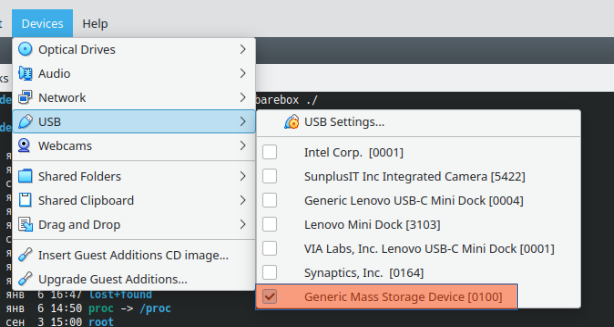
\includegraphics[width=\textwidth]{pic_04}
\end{center}

\subsection{}Необходимо узнать точку монтирования SD карты. Она может отличаться в зависимости от ридера. Для упрощения ввода, выполните команду в консоле:
\begin{lstlisting}[style=bash]
	# mount | grep ^/dev
\end{lstlisting}
для получения списка примонтированных устройств, при этом командой grep происходит фильтрация лишнего вывода, и отображается только список блочных устройств. Вывод будет примерно как на рисунке

\begin{center}
	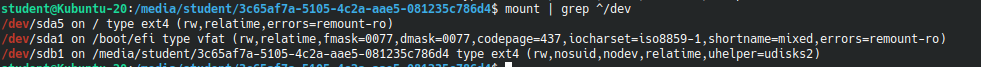
\includegraphics[width=\textwidth]{pic_05}
\end{center}

Первые две строчки, это разделы виртуального жёсткого диска, далее точка монтирования SD карты (/media/student/…)

Для упрощения ввода, создадим временную системную переменную, которой назначим путь, для примера\textbf{(!)} на рисунке выше:
\begin{lstlisting}[style=bash]
	# export BAGET_SD=\
	/media/student/3c65af7a-5105-4c2a-aae5-081235c786d4
\end{lstlisting}

Нужно помнить, что эта переменная существует только в том терминале, где был вызван export, в остальных окнах терминала она не существует, если Вы закроете текущее окно, или Вам понадобиться эта переменная в другом окне, необходимо будет повторить процедуру присвоения.

\subsection{}Удалите все файлы с sd карты
\begin{lstlisting}[style=bash]
	# sudo rm -rf $BAGET_SD/*
\end{lstlisting}
скопируйте созданную rootfs на sd карту
\begin{lstlisting}[style=bash]
	# sudo cp -a $BAGET/lab_01/rootfs/* $BAGET_SD/
\end{lstlisting}
и отмантируйте SD карту 
\begin{lstlisting}[style=bash]
	# sudo umount $BAGET_SD
\end{lstlisting}
(это важно, так как в ОС Linux запись данных на носители происходит в фоне, и если вы отключите накопитель «неправильно» то нет гарантии, что данные успели записаться на носитель!).
Дождитесь когда команда выполниться, после чего достаньте SD карту и вставьте её в плату.

\subsection{}Подключите USB шнуром плату к ПК. Проверьте, и при необходимости подключите USB устройство FTDI RBM\_C1K5500VK018 к виртуальной машине (меню Device→USB).

\subsection{} Запустите программу gtkterm 

\subsection{} Выберите порт /dev/ttyUSB1 

Если в окне не появился текст, и на нажатие клавиши Enter так же нет реакции,  нажмите на кнопку Reset на плате. Изучите вывод, там будет написано, что пошло не так.

Один из вариантов, когда при записи файлов на SD карту что-то побилось. В этом случае, увидите много записей как в примере ниже:
\begin{lstlisting}[style=stdout]
	srisa-sdhci 1b50b000.sdhci@1b50b000.of: registered as mci0
	srisa-sdhci 1b50b000.sdhci@1b50b000.of: SDHCI timeout while waiting for done
	srisa-sdhci 1b50b000.sdhci@1b50b000.of: error on command 8
	srisa-sdhci 1b50b000.sdhci@1b50b000.of: state = 0400 03ff, interrupt = 8001 0001
	srisa-sdhci 1b50b000.sdhci@1b50b000.of: r0 00000000 r1 00000000 r2 00000000 r3 00000000
\end{lstlisting}

Нужно повторить все шаги этого раздела. \textbf{При вынимании SD карты убедитесь, что плата обесточена!}

\section{Проверка}

\subsection{}Проверьте, что сервис apache2 работает. 
\begin{lstlisting}[style=bash]
$ ps -aux | grep apache2
\end{lstlisting}
\begin{center}
	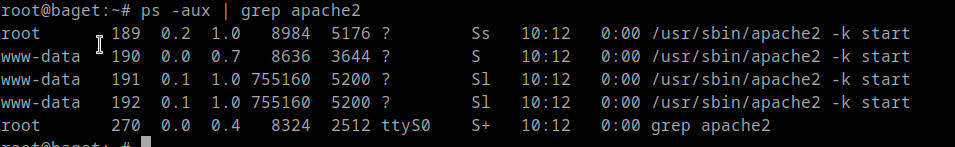
\includegraphics[width=\textwidth]{pic_23}
\end{center}

\subsection{}После чего откройте браузер в виртуальной машине, и вбейте в адресное поле ip адрес платы (192.168.100.200) вы должны поучить страницу, как на рисунке ниже
\begin{center}
	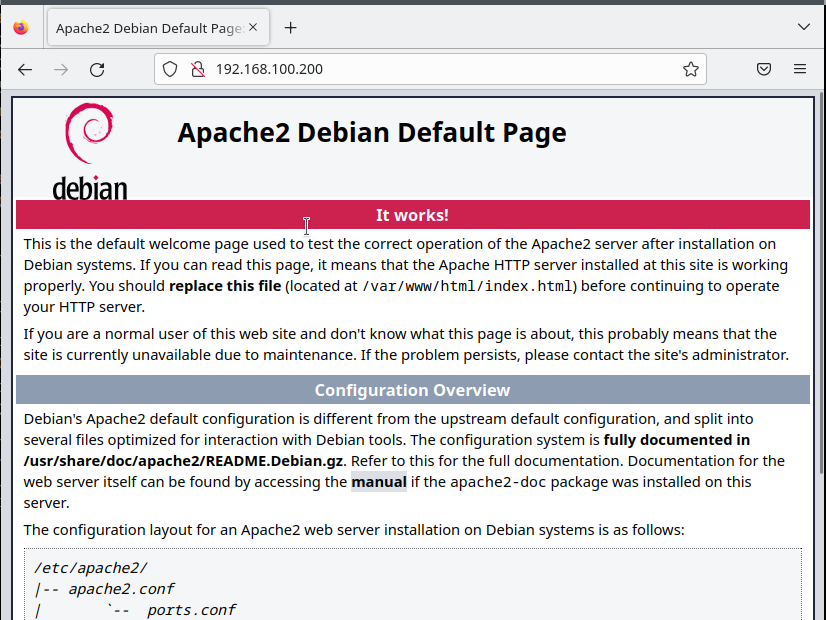
\includegraphics[width=\textwidth]{pic_24}
\end{center}
\textbf{Замечание:} если вы получили результат, что страница не найдена, проверьте, что у адреса префикс http и повторите попытку снова. Помните, если браузер не находит ответа от http, он автоматически переключается на https и пробует найти что-то там. А так как префикс определяет порт, к которому отправляются запросы (https это 433 порт), то важно убедиться, что браузер пытается подключиться к нужному порту (в конфигурация описан только 80 порт).

\subsection{}В терминале платы, запустите сокет, для управления светодиодами 
\begin{lstlisting}[style=bash]
$ python3 /var/www/led_socekt.py &
\end{lstlisting}

\subsection{}Откройте в браузере страницу admin.html: 192.168.100.200/admin.html
вы должны увидеть страницу следующего вида
\begin{center}
	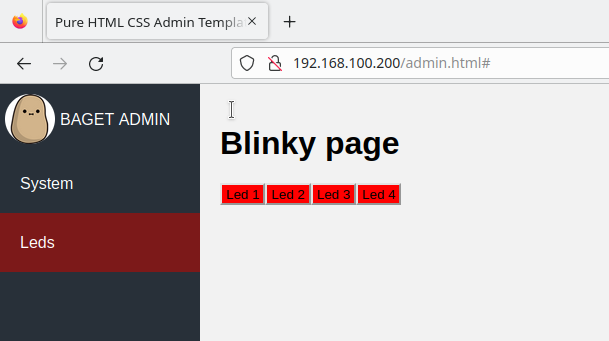
\includegraphics[width=\textwidth]{pic_25}
\end{center}

Первый пункт, будет выдавать информацию о плате (свободное место на диске, загруженность процессора, и RAM памяти, IP адреса платы).

Второй пункт позволяет управлять светодиодами, подключённым к первым четырём выводам банка выводов F.

Нужно понимать, что веб-сервер в системе работает, как ещё один терминал (вспомните, как подключались к терминалу платы по ssh, тут нечто похожее). При этом подключение ведётся не от имени суперпользователя (так делать никогда нельзя, если конечно не хотите сделать большой проход в систему). Мало того, этот «пользователь», не может получить доступа к корневому каталогу платы, для него корневым каталогом в является папка /var/www/ (в текущих конфигурация сервера).

Так же, можно заметить, что при попытке управлять светодиодами, возникает большая задержка, между тем как происходит нажатие кнопки на веб-странице и непосредственно переключением светодиода. Это связано с тем, что CGI технология не самая быстрая, и в современности применяется FastCGI или uWSGI. Однако их настройка более комплексная, чем CGI, поэтому в рамках данной лабораторной работы не рассматривалась.   

\subsection{} Выключите плату, для чего в начале введите команду
\begin{lstlisting}[style=bash]
	$ poweroff
\end{lstlisting}
дождитесь, как появиться надпись
\begin{lstlisting}[style=stdout]
	reboot: System halt
\end{lstlisting}
после чего отключите USB кабель от ПК или платы. 

\section{Задание для самостоятельной работы}
Добавте возможность управления всеми выводами банка F. Можно воспользоватся тектовым редактором nano установленном на целевой платформе.

Необходимо внести правки в следующие файлы:
\begin{itemize}
	\item led\_socekt.py - дописать элементы в строке 6 (если фалй уже запускался, остановите его выполнение командой killall python3, и не запустие его вновь, после редактирования)
	
	\item /var/www/js/led\_ctrl.js - дописать в первой строке ещё 4 элемента, для проверки достаточно обновить страницу в браузере. Дополнительно, можно посмотреть отладочную информацию кликнув правой клавишей мыши на странице и выбрав пункт Inspect. В открывшемся наборе вкладок выберите Console. Если в результате правок были допущены ошибки, тут будет о них информация. 
	
	
\end{itemize} 